\documentclass[runningheads]{llncs}

% ---------------------------------------------------------------
% Include basic ECCV package
\usepackage[review,year=2026,ID=7581]{eccv}

% ---------------------------------------------------------------
% Other packages
\usepackage{eccvabbrv}
\usepackage{graphicx}
\usepackage{booktabs}
\usepackage{mathtools}
\usepackage{amsmath}
\usepackage{amssymb}
\usepackage{algorithm}
\usepackage{algorithmic}
\usepackage{multirow}
\usepackage{xcolor}
\usepackage[accsupp]{axessibility}
\usepackage{hyperref}

% Custom commands (same as main paper)
\newcommand{\method}{FreshPER}
\newcommand{\R}{\mathbb{R}}
\newcommand{\E}{\mathbb{E}}
\newcommand{\piold}{\pi_{\text{old}}}
\newcommand{\pinew}{\pi_{\theta}}

\begin{document}

\title{Supplementary Material: Freshness-Aware Prioritized Experience Replay for LLM/VLM Reinforcement Learning}

\titlerunning{Supplementary: Freshness-Aware PER for LLM/VLM RL}

\author{Anonymous Authors}
\authorrunning{Anonymous Authors}
\institute{Anonymous Institution}

\maketitle

\setcounter{section}{0}
\renewcommand{\thesection}{\Alph{section}}

\section{System Design Details}
\label{app:system}

\subsection{Replay Buffer Architecture}
\label{app:buffer_arch}

The replay buffer operates at the \emph{trajectory level}: each entry stores a complete episode (prompt, all assistant turns, and environment observations) along with its behavior log-probabilities, reward, collection step~$t_i$, and current priority~$p_i$. This granularity naturally matches agentic RL, where episode-level rewards are the primary training signal.

When the buffer reaches capacity, we evict the entry with the lowest effective priority---i.e., the oldest, lowest-priority trajectory---which follows naturally from the age decay: entries whose priority has decayed near zero are evicted first. The priority refresh step (Line~5 of Algorithm~1 in the main paper) recomputes all priorities with current ages once per iteration. To avoid blocking the training loop, this $O(N)$ scan runs in a background CPU thread during on-policy GPU training, completing in $50$--$100$\,ms for $N{=}100$K entries and fully overlapping with GPU computation.

\subsection{Framework Integration}
\label{app:pipeline}

We implement \method{} on top of the ROLL framework~\cite{wang2025roll}, which provides a single-controller architecture that decouples inference and training across GPU pools. The replay buffer and all priority logic run on the CPU-side controller, naturally pipelining with GPU-bound training and inference. The training flow follows Algorithm~1 in the main paper: fresh rollouts are first used for on-policy training, then stored into the buffer; the replay loop draws prioritized batches for $K$ additional off-policy updates per environment interaction.


\section{Additional Ablation Studies}
\label{app:ablations}

\subsection{Age Decay Constant $\tau$}
\label{app:tau_ablation}

We ablate $\tau \in \{500, 1000, 1500\}$ on Sokoban Simple and FrozenLake (LLM, 0.5B), comparing against On-Policy and Standard PER (equivalent to $\tau{=}\infty$).

\begin{figure}[htb]
\centering
\begin{minipage}[b]{0.48\linewidth}
    \centering
    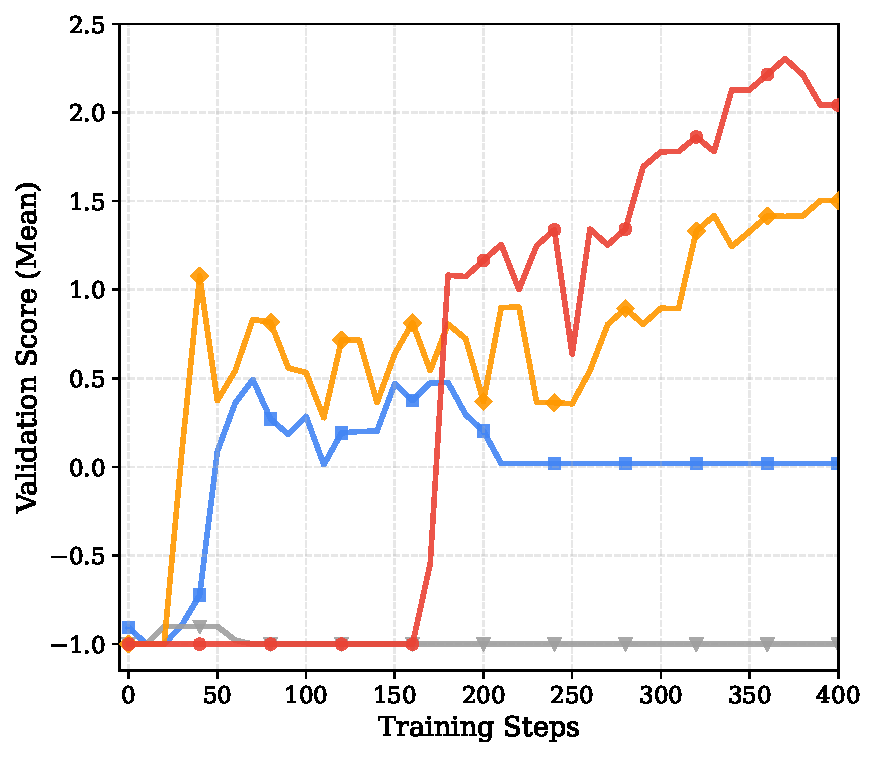
\includegraphics[width=\linewidth]{figures/llm/sokoban_age_decay_ablation.pdf}
    \\ {\small (a) Sokoban Simple}
\end{minipage}
\hfill
\begin{minipage}[b]{0.48\linewidth}
    \centering
    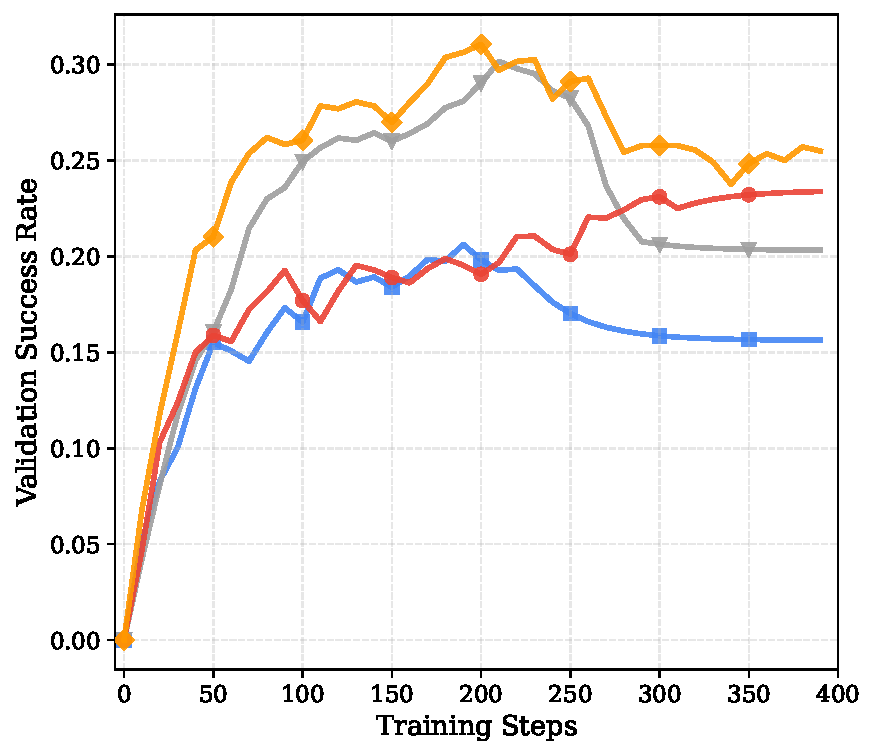
\includegraphics[width=\linewidth]{figures/llm/frozen_lake_age_decay_ablation.pdf}
    \\ {\small (b) FrozenLake (LLM)}
\end{minipage}
\caption{Ablation of age decay constant $\tau$. {\color[HTML]{4285F4}Blue~$\blacksquare$}: Baseline; {\color[HTML]{EA4335}Red~$\bullet$}: $\tau{=}500$; {\color[HTML]{FF9800}Orange~$\blacklozenge$}: $\tau{=}1000$; {\color[HTML]{9E9E9E}Gray~$\blacktriangledown$}: $\tau{=}1500$.}
\label{fig:supp_tau_ablation}
\end{figure}

On Sokoban Simple (\cref{fig:supp_tau_ablation}a), $\tau{=}500$ achieves a peak score of 2.30, $\tau{=}1000$ reaches 1.50, and $\tau{=}1500$ completely fails ($-$0.90), identical to Standard PER. This environment exhibits rapid policy drift, requiring aggressive decay. On FrozenLake (\cref{fig:supp_tau_ablation}b), the ranking shifts: $\tau{=}1000$ achieves the highest peak (0.336), followed by $\tau{=}1500$ (0.328) and $\tau{=}500$ (0.266). Unlike Sokoban, even $\tau{=}1500$ remains effective, indicating that FrozenLake tolerates higher data staleness.

\subsection{Importance Sampling Correction}
\label{app:is_ablation}

We investigate whether importance sampling (IS) correction improves training stability when combined with freshness decay. We compare $\tau{=}500$ with and without IS ($\beta{=}0.4$) on FrozenLake.

\begin{figure}[htb]
    \centering
    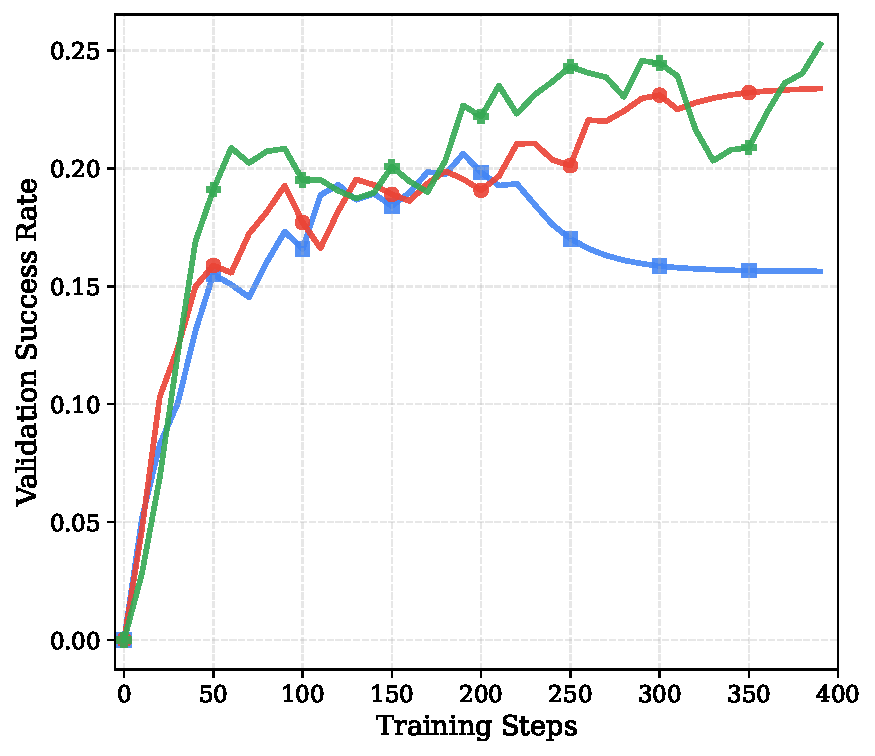
\includegraphics[width=0.55\linewidth]{figures/llm/frozen_lake_is_ablation.pdf}
    \caption{IS correction ablation on FrozenLake (LLM). {\color[HTML]{4285F4}Blue~$\blacksquare$}: Baseline; {\color[HTML]{EA4335}Red~$\bullet$}: $\tau{=}500$; {\color[HTML]{34A853}Green~$\boldsymbol{+}$}: $\tau{=}500$ + IS.}
    \label{fig:supp_is_ablation}
\end{figure}

\cref{fig:supp_is_ablation} shows that IS correction does not substantially boost peak performance ($+$5.9\%, from 0.266 to 0.281), but its primary value lies in \emph{training stability}: the IS variant is the only configuration whose final performance equals its peak (0.281 at both step~40 and step~390), whereas all other methods degrade in late training. This complementarity---freshness decay improves peak performance by suppressing stale priorities, while IS correction stabilizes training by compensating for distribution shift---validates the modular design of \method{}, where age decay and IS correction can be independently activated based on task requirements.

\subsection{When Does Replay Help?}
\label{app:control}

To understand the boundary conditions of \method{}, we evaluate on two environments where replay is expected to offer little benefit.

\begin{figure}[htb]
\centering
\begin{minipage}[b]{0.48\linewidth}
    \centering
    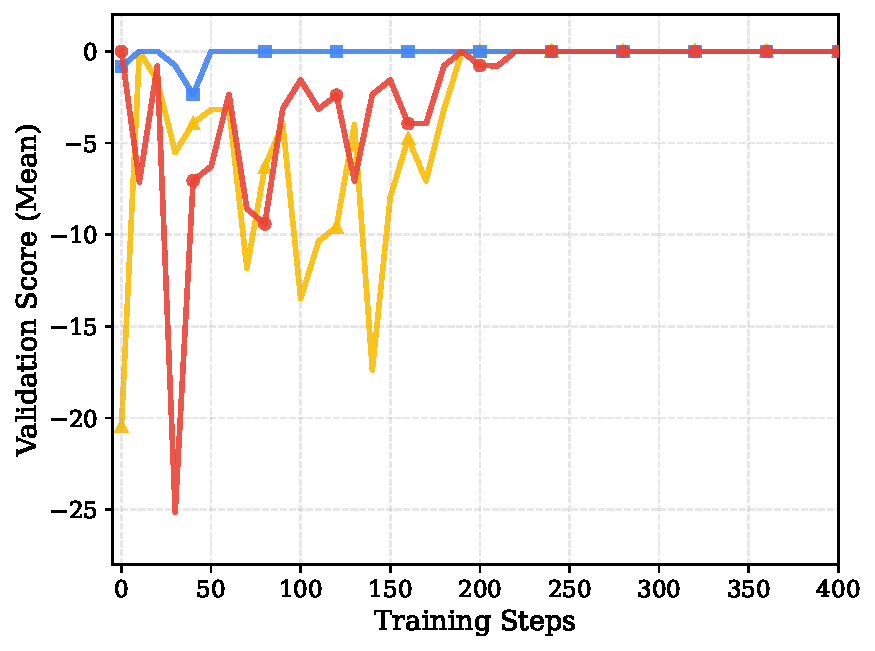
\includegraphics[width=\linewidth]{figures/llm/cliffwalking.pdf}
    \\ {\small (a) CliffWalking}
\end{minipage}
\hfill
\begin{minipage}[b]{0.48\linewidth}
    \centering
    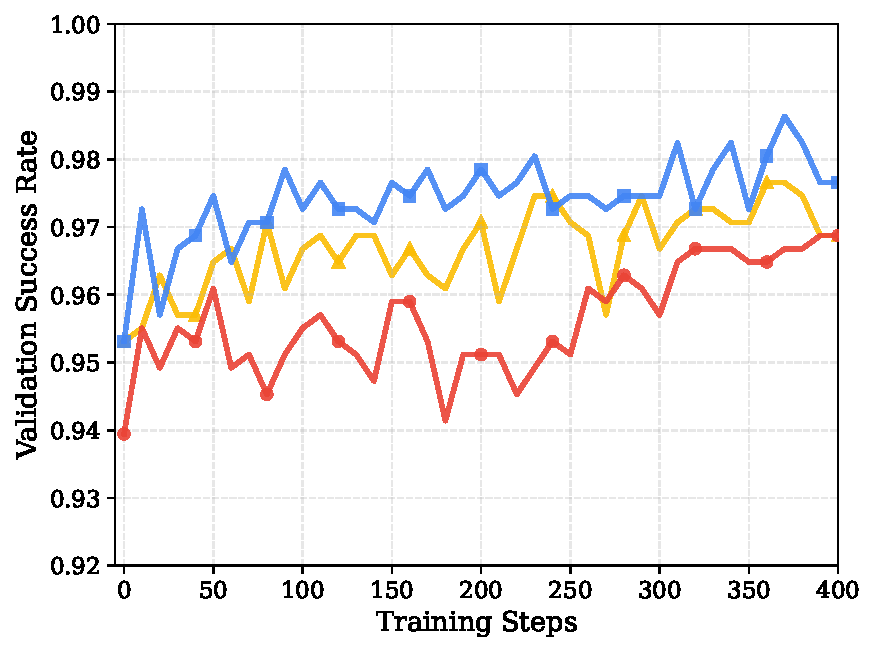
\includegraphics[width=\linewidth]{figures/llm/gsm8k.pdf}
    \\ {\small (b) GSM8K}
\end{minipage}
\caption{Control experiments. {\color[HTML]{4285F4}Blue~$\blacksquare$}: On-Policy; {\color[HTML]{FBBC04}Yellow~$\blacktriangle$}: Standard PER; {\color[HTML]{EA4335}Red~$\bullet$}: \method{} (Ours).}
\label{fig:supp_control}
\end{figure}

\paragraph{Too-Simple Environments (CliffWalking).}
All three methods converge to the optimal score of 0 (\cref{fig:supp_control}a). On-Policy converges fastest and most stably, while Standard PER and \method{} exhibit transient instability (PER shows spikes down to $-$17 at step~140). When the task is simple enough for on-policy training to solve quickly, replay provides no benefit and may introduce unnecessary off-policy noise.

\paragraph{Near-Saturated Models (GSM8K).}
All methods cluster in the narrow 0.94--0.99 range (\cref{fig:supp_control}b). The base model already achieves 93--95\% success; training provides only ${\sim}$2--3\% additional improvement. With so little room for improvement, replay-based methods cannot demonstrate meaningful advantages.

These control experiments delineate the regime where \method{} is most valuable: tasks that are \emph{challenging enough} that on-policy training either converges slowly or collapses, and where the model has \emph{sufficient room for improvement}.

\section{Derivations for Priority Staleness}
\label{app:staleness_derivation}

This section provides detailed derivations for the results stated in Section~3.3 of the main paper.

% ---------------------------------------------------------------------
\subsection{Variance of Importance Weights Equals \texorpdfstring{$\chi^2$}{Chi-squared}-Divergence}
\label{app:var_chi2}

\begin{proposition}
\label{prop:var_chi2}
Let $P$ and $Q$ be two probability distributions with $Q$ absolutely continuous with respect to $P$, and let $\rho(x) = P(x)/Q(x)$ denote the importance ratio. Then
\begin{equation}
    \mathrm{Var}_{Q}[\rho] = \chi^2(P \| Q),
\end{equation}
where $\chi^2(P\|Q) = \mathbb{E}_Q\!\left[(\rho - 1)^2\right]$ is the $\chi^2$-divergence.
\end{proposition}

\begin{proof}
By the definition of variance:
\begin{equation}
    \mathrm{Var}_{Q}[\rho]
    = \mathbb{E}_{Q}[\rho^2] - \left(\mathbb{E}_{Q}[\rho]\right)^2.
    \label{eq:app_var_def}
\end{equation}
We first evaluate the mean of $\rho$ under $Q$:
\begin{equation}
    \mathbb{E}_{Q}[\rho]
    = \int Q(x) \cdot \frac{P(x)}{Q(x)} \, dx
    = \int P(x) \, dx
    = 1,
    \label{eq:app_rho_mean}
\end{equation}
where the last equality holds because $P$ is a valid probability distribution. Substituting into Eq.~\eqref{eq:app_var_def}:
\begin{equation}
    \mathrm{Var}_{Q}[\rho]
    = \mathbb{E}_{Q}[\rho^2] - 1.
    \label{eq:app_var_simplified}
\end{equation}

Now expand the $\chi^2$-divergence from its definition:
\begin{equation}
    \chi^2(P \| Q)
    = \mathbb{E}_{Q}\!\left[(\rho - 1)^2\right]
    = \mathbb{E}_{Q}[\rho^2] - 2\,\mathbb{E}_{Q}[\rho] + 1
    = \mathbb{E}_{Q}[\rho^2] - 1,
    \label{eq:app_chi2_expanded}
\end{equation}
where we again used $\mathbb{E}_Q[\rho] = 1$. Comparing Eq.~\eqref{eq:app_var_simplified} and Eq.~\eqref{eq:app_chi2_expanded} completes the proof.
\end{proof}

% ---------------------------------------------------------------------
\subsection{Monotonicity of R\'{e}nyi Divergence and the \texorpdfstring{$D_2 \geq D_{\mathrm{KL}}$}{D2 >= DKL} Bound}
\label{app:renyi_mono}

The R\'{e}nyi divergence of order $\alpha > 0$ ($\alpha \neq 1$) between distributions $P$ and $Q$ is defined as:
\begin{equation}
    D_\alpha(P \| Q)
    = \frac{1}{\alpha - 1}\,\log \mathbb{E}_{Q}\!\left[\left(\frac{P(x)}{Q(x)}\right)^{\!\alpha}\right].
    \label{eq:app_renyi_def}
\end{equation}
Two standard properties are relevant here:

\paragraph{Property 1: Connection to $\chi^2$-divergence.}
Setting $\alpha = 2$ in Eq.~\eqref{eq:app_renyi_def}:
\begin{equation}
    D_2(P \| Q)
    = \log \mathbb{E}_{Q}\!\left[\rho^2\right]
    = \log\!\left(1 + \chi^2(P \| Q)\right),
    \label{eq:app_d2_chi2}
\end{equation}
where we used $\mathbb{E}_Q[\rho^2] = 1 + \chi^2$ from Eq.~\eqref{eq:app_chi2_expanded}. Rearranging:
\begin{equation}
    \chi^2(P \| Q) = \exp\!\left(D_2(P \| Q)\right) - 1.
    \label{eq:app_chi2_from_d2}
\end{equation}

\paragraph{Property 2: Monotonicity in $\alpha$.}
Previous studies \cite{van_Erven_2014} have demonstrated that $D_\alpha(P\|Q)$ is non-decreasing in $\alpha$. The KL divergence is recovered in the limit $\alpha \to 1$:
\begin{equation}
    D_{\mathrm{KL}}(P \| Q) = \lim_{\alpha \to 1}\, D_\alpha(P \| Q).
\end{equation}
Since $\alpha = 2 > 1$, monotonicity immediately gives:
\begin{equation}
    D_2(P \| Q) \;\geq\; D_{\mathrm{KL}}(P \| Q).
    \label{eq:app_d2_geq_kl}
\end{equation}

Combining Eq.~\eqref{eq:app_chi2_from_d2} and Eq.~\eqref{eq:app_d2_geq_kl}, and using the monotonicity of the exponential:
\begin{equation}
    \mathrm{Var}_Q[\rho]
    = \chi^2(P \| Q)
    = \exp(D_2) - 1
    \;\geq\; \exp(D_{\mathrm{KL}}) - 1.
    \label{eq:app_var_lower_bound}
\end{equation}

% ---------------------------------------------------------------------
\subsection{Effective Sample Size Decay}
\label{app:ess_derivation}

The effective sample size (ESS)~\cite{kong1992note} quantifies how many of $n$ importance-weighted samples are effectively contributing to an estimate. Formally:
\begin{equation}
    \mathrm{ESS} = \frac{n}{1 + \mathrm{Var}_{Q}[\rho]}.
    \label{eq:app_ess_def}
\end{equation}
When $\pi_\theta = \pi_\mu$ (i.e., $\rho \equiv 1$, $\mathrm{Var}[\rho] = 0$), all samples are equally useful and $\mathrm{ESS} = n$. As $\mathrm{Var}[\rho]$ grows, more samples are effectively wasted and the ESS shrinks.

Substituting the lower bound from Eq.~\eqref{eq:app_var_lower_bound}:
\begin{equation}
    \mathrm{ESS}
    = \frac{n}{1 + \mathrm{Var}[\rho]}
    \leq \frac{n}{1 + \exp(D_{\mathrm{KL}}) - 1}
    = \frac{n}{\exp(D_{\mathrm{KL}})}.
    \label{eq:app_ess_step1}
\end{equation}
This shows that per-sample effective contribution decays exponentially with the KL divergence between the two policies.

\section{Environment and Model Details}
\label{app:env}

Table~\ref{tab:env_details} summarizes the eight evaluation environments. We use three model scales across experiments, chosen to match the computational cost of each task.

\begin{table}[ht]
\scriptsize
\caption{Environment and model configurations. ``Max Actions'' denotes the maximum number of assistant turns per episode. ``Seq Len'' is the maximum sequence length (prompt + all turns). ``Config'' refers to the hyperparameter configuration (Section~\ref{app:config_a}).}
\label{tab:env_details}
\begin{tabular}{llcccccl}
    \toprule
    \textbf{Environment} & \textbf{Type} & \textbf{Model} & \textbf{GPUs} & \textbf{Seq Len} & \textbf{Max Actions} & \textbf{Config} & \textbf{Reward} \\
    \midrule
    NQ Search & LLM & Qwen2.5-7B & 8 & 12800 & 5 & Default & Binary (EM) \\
    AIME & LLM & Qwen2.5-7B & 8 & 4096 & 3 & A & Binary \\
    Sokoban Simple & LLM & Qwen2.5-0.5B & 2 & 2048 & 10 & A & $[-1, +3]$ \\
    Sokoban Hard & LLM & Qwen2.5-0.5B & 2 & 2048 & 10 & A & $[-1, +3]$ \\
    FrozenLake (LLM) & LLM & Qwen2.5-0.5B & 2 & 2048 & 10 & A & Binary \\
    CliffWalking & LLM & Qwen2.5-0.5B & 2 & 2048 & 200 & A & $[-\infty, 0]$ \\
    GSM8K & LLM & Qwen2.5-0.5B & 2 & 4096 & 3 & A & Binary \\
    \midrule
    FrozenLake (VLM) & VLM & Qwen2.5-VL-3B & 4 & 4096 & 10 & Default & Binary \\
    GeoQA & VLM & Qwen2.5-VL-3B & 4 & 4096 & 3 & Default & Binary \\
    \bottomrule
\end{tabular}
\end{table}

\paragraph{NQ Search.}
An agentic retrieval-augmented QA task on Natural Questions~\cite{jin2025searchr1}. The agent alternates between reasoning (\texttt{<think>}), issuing search queries (\texttt{<search>}), and producing a final answer (\texttt{<answer>}). Retrieved documents are provided via a FAISS index with E5 embeddings ($k{=}3$ passages per query). Reward is binary exact-match (EM), with case/punctuation/article normalization. The long sequence length (12800 tokens) accommodates multi-turn search context.

\paragraph{AIME.}
A math competition task based on the American Invitational Mathematics Examination. We use 90 AIME I/II problems from 2022--2024 (30 per year) from the AI-MO validation AIME set~\cite{aimoValidationAime}, whose entries link to the Art of Problem Solving archive~\cite{aopsAimeArchive}. Each problem requires an integer answer in the range 000--999. The agent has up to 3 attempts per problem; if the first answer is incorrect, it receives feedback and may try again. Reward is binary (correct/incorrect). We use Qwen2.5-7B-Instruct with Config~A ($\tau{=}1000$) on 8 GPUs.

\paragraph{Sokoban.}
A box-pushing puzzle on a grid where the agent must push all boxes onto target positions~\cite{wang2025roll}. Actions are irreversible---a misplaced box cannot be pulled back. We evaluate two difficulty levels: \emph{Simple} ($6{\times}6$ grid, 1~box) and \emph{Hard} (larger layouts, more boxes). Score ranges from $-1$ (all boxes misplaced) to $+3$ (all on target), making it a dense reward signal with a meaningful performance gradient.

\paragraph{FrozenLake (LLM).}
A text-only navigation task on a $4{\times}4$ grid with slippery ice. The agent receives a text description of the grid state and must navigate to the goal while avoiding holes. Slippery dynamics mean the agent moves in the intended direction with probability $1/3$ and slides sideways otherwise, making the task stochastic. Used for both main evaluation and ablation studies.

\paragraph{CliffWalking.}
A $4{\times}12$ grid navigation task where the agent must reach the goal while avoiding a cliff along the bottom row. Falling off the cliff incurs a large negative reward ($-100$) and resets the agent. The optimal policy achieves score~0. This serves as a control: the task is simple enough that on-policy training solves it quickly, and replay is not expected to help.

\paragraph{GSM8K.}
Grade-school math word problems~\cite{cobbe2021gsm8k} requiring multi-step arithmetic reasoning. The base Qwen2.5-0.5B model already achieves ${>}$93\% accuracy on this task, so it serves as a near-saturated control where replay cannot provide meaningful improvements.

\paragraph{FrozenLake (VLM).}
The visual counterpart of the text FrozenLake: the $4{\times}4$ grid is rendered as an RGB image, and the VLM agent must interpret the visual state to navigate. This tests whether \method{} generalizes to multimodal settings where observations are images rather than text.

\paragraph{GeoQA.}
A geometry question-answering task~\cite{chen2021geoqa} where the VLM interprets geometric diagrams and solves problems requiring spatial reasoning. Binary reward (correct/incorrect).


\section{Engineering Insights: Hyperparameter Configuration for Off-Policy LLM RL}
\label{app:config_a}

During development, we discovered that standard on-policy hyperparameters are unsuitable for off-policy training with a replay buffer. We summarize the key findings below, as they may benefit practitioners adopting experience replay for LLM RL.

\paragraph{Advantage Clipping is Critical.}
The default advantage clipping threshold in many LLM RL implementations is large ($\epsilon_{\text{clip}} = 20$), effectively disabling clipping. For on-policy training this is harmless, but with replay data, stale trajectories can produce extreme advantage values that destabilize training. We found that reducing the clip to $\epsilon_{\text{clip}} = 0.2$---the same value used for the PPO ratio clip---was essential for stable off-policy learning. With $\epsilon_{\text{clip}} = 20$, replay-augmented training frequently diverged; with $\epsilon_{\text{clip}} = 0.2$, it was consistently stable across all environments.

\paragraph{KL Regularization Should Be Disabled.}
On-policy methods commonly use KL divergence penalties ($\beta_{\text{KL}} = 0.05$--$0.1$) to prevent the policy from deviating too far from the reference model. However, with off-policy replay, the KL penalty interacts poorly with stale data: old trajectories already have large KL divergence from the reference, and penalizing this further suppresses useful gradient signal from replay. We found that setting $\beta_{\text{KL}} = 0$ (and disabling the adaptive KL controller) improved performance across all environments when using a replay buffer.

\paragraph{Entropy Bonus is Unnecessary.}
Similarly, the entropy loss coefficient ($\lambda_{\text{ent}} = 0.01$) commonly used for exploration in on-policy training was counterproductive with replay. The replay buffer itself provides exploration diversity; adding an entropy bonus on top led to overly stochastic policies.

Table~\ref{tab:config_comparison} summarizes these differences. We refer to the off-policy-optimized configuration as ``Config~A'' throughout our experiments.

\begin{table}[ht]
\centering
\caption{Hyperparameter comparison between standard on-policy settings and our off-policy-optimized Config~A.}
\label{tab:config_comparison}
\small
\begin{tabular}{lcc}
    \toprule
    \textbf{Parameter} & \textbf{On-Policy (Default)} & \textbf{Config~A (Off-Policy)} \\
    \midrule
    Advantage clip $\epsilon_{\text{clip}}$ & 20 & \textbf{0.2} \\
    KL loss enabled & \checkmark & $\times$ \\
    KL coefficient $\beta_{\text{KL}}$ & 0.05--0.1 & \textbf{0.0} \\
    Init KL coefficient & 0.1 & \textbf{0.0} \\
    Entropy coefficient $\lambda_{\text{ent}}$ & 0.01 & \textbf{0.0} \\
    PPO epochs & 1 & 1 \\
    Max gradient norm & 1.0 & 1.0 \\
    Advantage estimator & REINFORCE++ & REINFORCE++ \\
    Whiten advantages & \checkmark & \checkmark \\
    \bottomrule
\end{tabular}
\end{table}

\noindent\textbf{Note}: Config~A was developed on FrozenLake (LLM, 0.5B) and subsequently validated on Sokoban, CliffWalking, and GSM8K without modification---all 0.5B experiments in this paper use Config~A for both baseline and replay runs. The NQ Search (7B) and VLM (3B) experiments use the default on-policy settings, as larger models appear more robust to these hyperparameter choices.


\section{Detailed Experimental Configurations}
\label{app:configs}

Table~\ref{tab:training_config} lists the full training configuration for each experiment family. All experiments use the ROLL framework~\cite{wang2025roll} with REINFORCE++ as the policy gradient algorithm, DeepSpeed for training, and vLLM for inference.

\begin{table}[ht]
\centering
\caption{Training configurations across experiment families. ``GA'' = gradient accumulation steps, ``BS/dev'' = per-device batch size. All experiments use learning rate $10^{-6}$.}
\label{tab:training_config}
\small
\begin{tabular}{lccccccc}
    \toprule
    \textbf{Experiment} & \textbf{Model} & \textbf{GPUs} & \textbf{BS/dev} & \textbf{GA} & \textbf{DeepSpeed} & \textbf{Max Steps} & \textbf{Config} \\
    \midrule
    NQ Search & 7B & 8 & 1 & 16 & ZeRO-3 & 300 & Default \\
    AIME & 7B & 8 & 2 & 32 & ZeRO-2 & 400 & A \\
    Sokoban & 0.5B & 2 & 4 & 32 & ZeRO-2 & 400 & A \\
    FrozenLake (LLM) & 0.5B & 2 & 4 & 32 & ZeRO-2 & 400 & A \\
    CliffWalking & 0.5B & 2 & 4 & 32 & ZeRO-2 & 400 & A \\
    GSM8K & 0.5B & 2 & 4 & 32 & ZeRO-2 & 400 & A \\
    \midrule
    FrozenLake (VLM) & VL-3B & 4 & 1 & 32 & ZeRO-2 & 100 & Default \\
    GeoQA & VL-3B & 4 & 1 & 32 & ZeRO-2 & 100 & Default \\
    \bottomrule
\end{tabular}
\end{table}

Table~\ref{tab:replay_config} details the replay buffer configuration. All replay-enabled experiments use a trajectory-level buffer with FIFO eviction and the same core priority parameters.

\begin{table}[ht]
\centering
\caption{Replay buffer configurations. All experiments use trajectory-level sampling, FIFO eviction, and priority exponent $\alpha{=}0.6$.}
\label{tab:replay_config}
\small
\begin{tabular}{lcccccc}
    \toprule
    \textbf{Method} & \textbf{Capacity} & \textbf{$K$} & \textbf{Priority} & \textbf{Age Decay $\tau$} & \textbf{IS ($\beta$)} \\
    \midrule
    On-Policy & --- & --- & --- & --- & --- \\
    Standard PER & 50K & 2 & $|r| + \epsilon$ & $\infty$ (disabled) & \checkmark~(0.4) \\
    \method{} (default) & 50K & 2 & $|r| + \epsilon$ & 500 & $\times$ \\
    \method{} ($\tau{=}1000$) & 50K & 2 & $|r| + \epsilon$ & 1000 & $\times$ \\
    \method{} ($\tau{=}1500$) & 50K & 2 & $|r| + \epsilon$ & 1500 & $\times$ \\
    \method{} ($\tau{=}500$, IS) & 50K & 2 & $|r| + \epsilon$ & 500 & \checkmark~(0.4) \\
    \bottomrule
\end{tabular}
\end{table}

\paragraph{Common Settings.}
All experiments share: rollout batch size 128, validation batch size 128, seed 42, cosine learning rate schedule with 10-step warmup, BF16 mixed precision, and FlashAttention-2. Inference uses vLLM with $\text{top-}p{=}0.99$, $\text{top-}k{=}100$, and temperature~0.99.

\paragraph{GPU Layout.}
For 2-GPU experiments (0.5B models): GPU~0 runs training (DeepSpeed) and reference model inference; GPU~1 runs vLLM inference. For 4-GPU experiments (VLM 3B): GPUs~0--1 run training and reference; GPUs~2--3 run vLLM. For 8-GPU experiments (NQ Search 7B): GPUs~0--3 run training (ZeRO-3); GPUs~4--7 run vLLM.


% ---- Bibliography ----
\bibliographystyle{splncs04}
\bibliography{main}

\end{document}
